\chapter{Vorlesung}
\section{Priority-Queue mittels Fibonacci-Heaps}
%Grafik1
\begin{figure}[h]
	\centering
	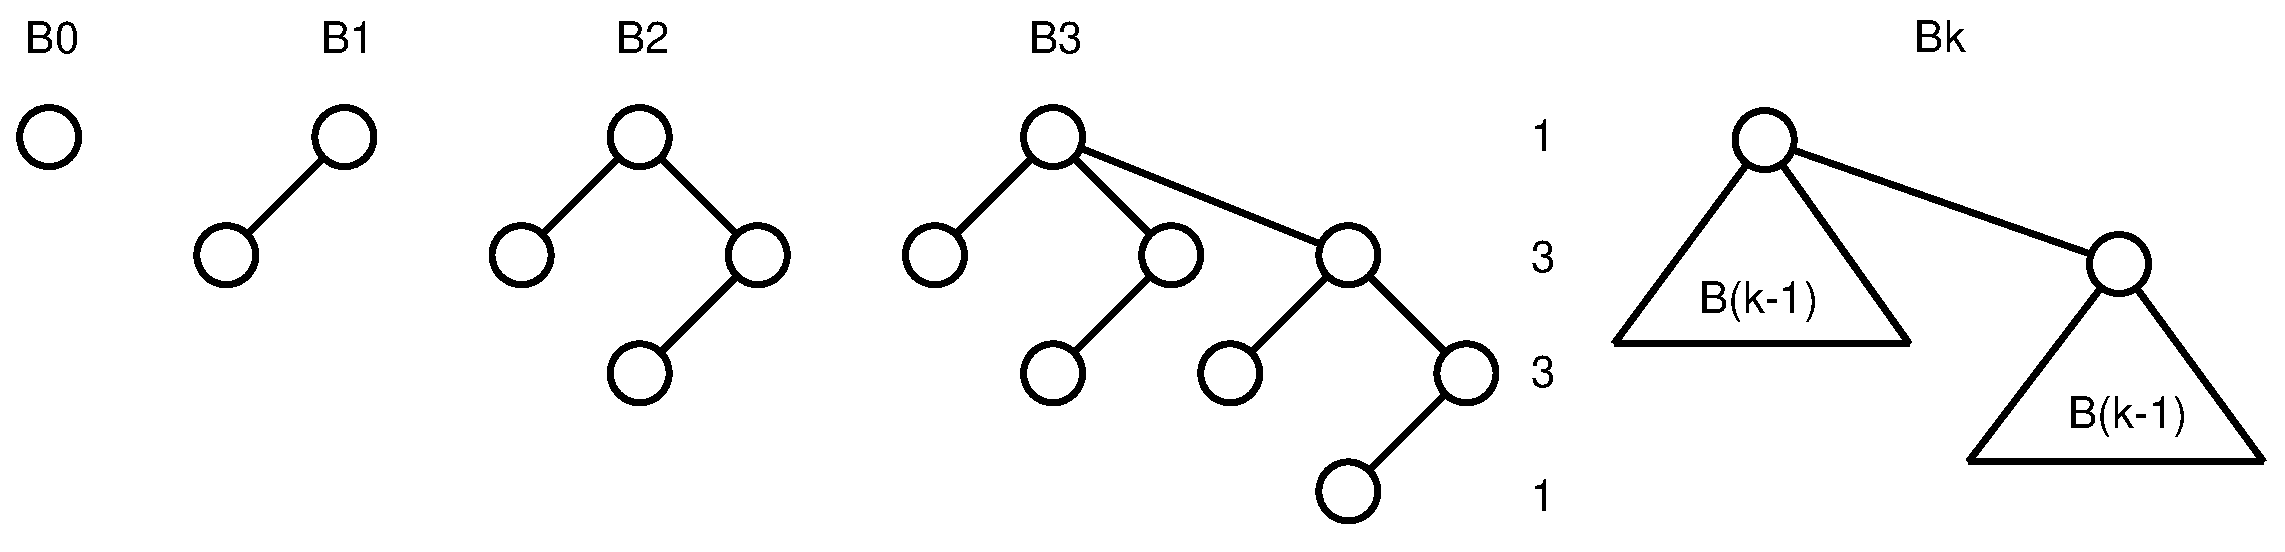
\includegraphics[width=0.65\linewidth]{21/Grafik/BinomialBaeume}
	\caption{Binomial-Bäume}
\end{figure}

Es gilt:\\
Zahl der Knoten auf Level $i$ ist $\binom{k}{i}$
\[  \binom{k}{i} = \binom{k-1}{i} + \binom{k-1}{i-1} \]
Gesamtzahl aller Knoten $=2^k$\\

%Pascal-Dreieck mit 5 Ebenen
\begin{tabular}{rccccccccc}
$n=0$:&    &    &    &    &  1\\\noalign{\smallskip\smallskip}
$n=1$:&    &    &    &  1 &    &  1\\\noalign{\smallskip\smallskip}
$n=2$:&    &    &  1 &    &  2 &    &  1\\\noalign{\smallskip\smallskip}
$n=3$:&    &  1 &    &  3 &    &  3 &    &  1\\\noalign{\smallskip\smallskip}
$n=4$:&  1 &    &  4 &    &  6 &    &  4 &    &  1\\\noalign{\smallskip\smallskip}
\end{tabular}


\subsection{Operationen eines Binomial-Heaps}

\begin{figure}[h]
	\centering
	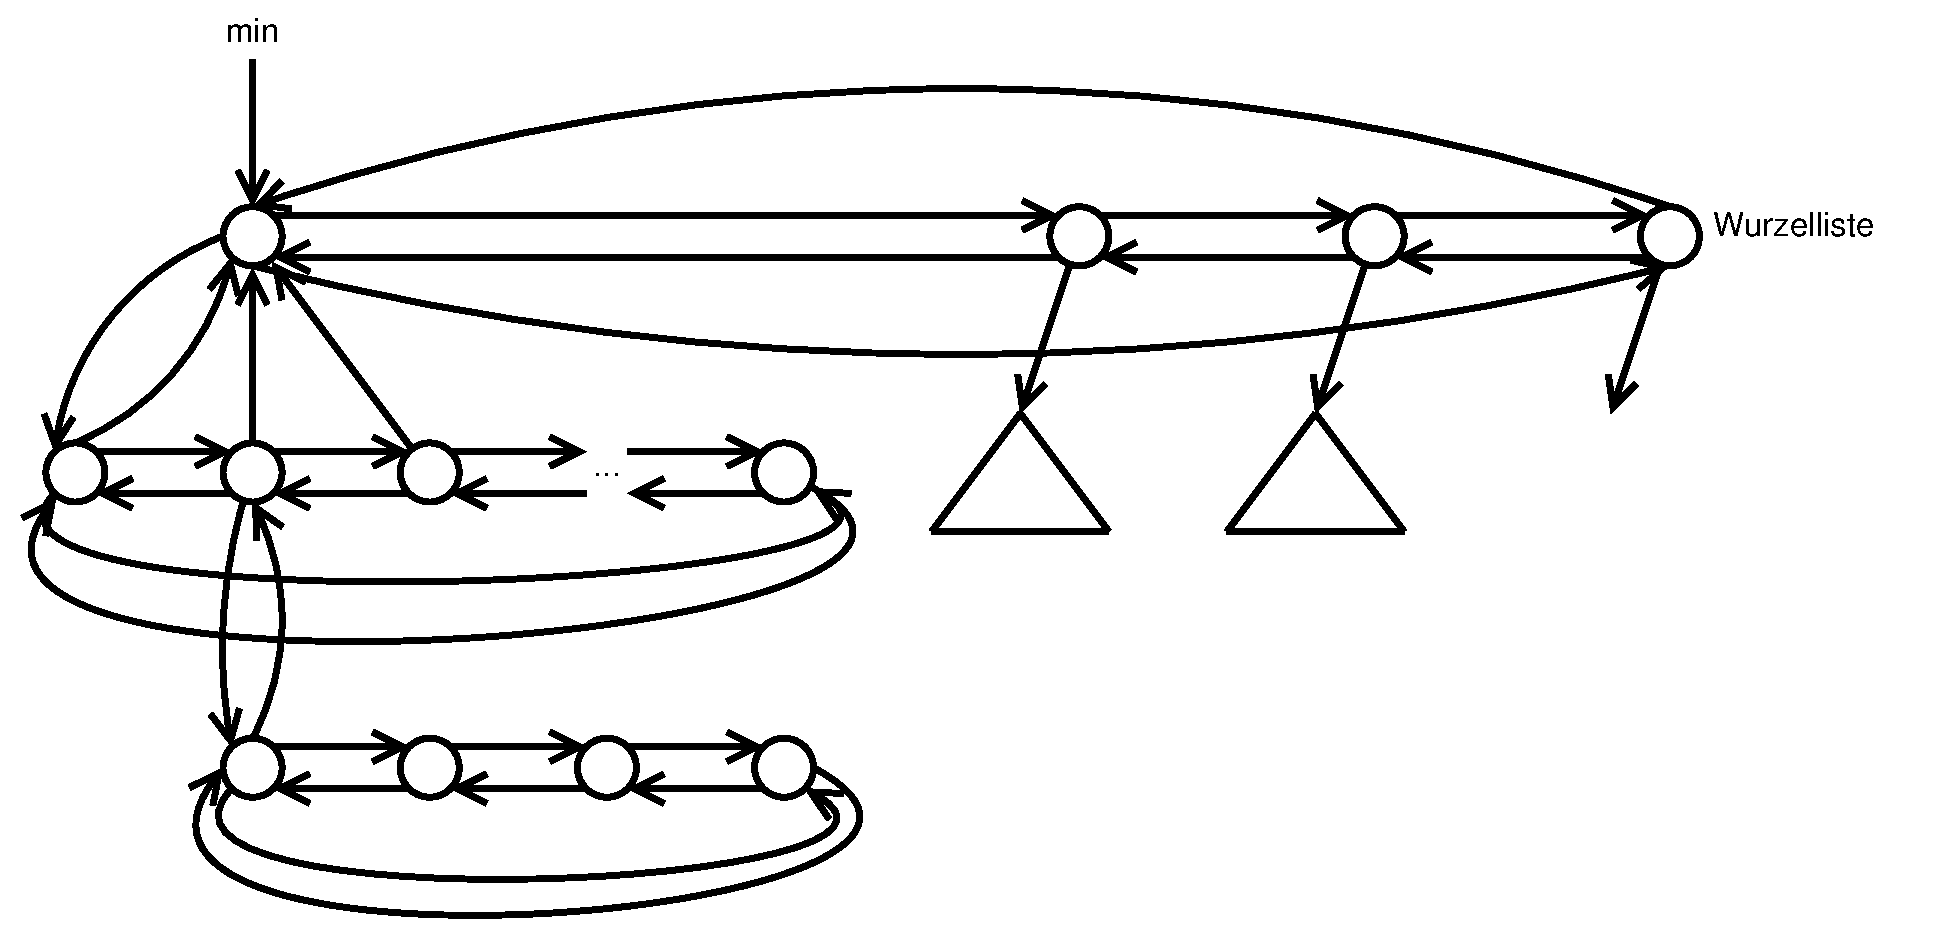
\includegraphics[width=0.65\linewidth]{21/Grafik/Aufbau}
	\caption{Aufbau}
\end{figure}

\begin{itemize}
	\item \texttt{insert}
	\item \texttt{deleteMin}
	\item \texttt{decreaseKey}
\end{itemize}

\paragraph{Idee}
Für jeden Knoten wird gelten, dass die Zahl aller Nachfahren $\geq \Phi^k~~k=$Knotengrad

\subsubsection{\texttt{Insert}}
Einzelner Knoten wird einfach in die Wurzelliste gehängt und Minimum wird aktualisiert.

\subsubsection{\texttt{DeleteMin}}
Lösche den Minimumsknoten und übernehme alle seine Kindknoten in die Wurzelliste. Konsolidiere anschließend die Wurzelliste. Nach dem Konsolidieren hat die Wurzelliste nur noch eine "`kleine"' Länge und wir bestimmen das neue Minimum durch einen Durchlauf durch diese Liste.
\begin{figure}[H]
	\centering
	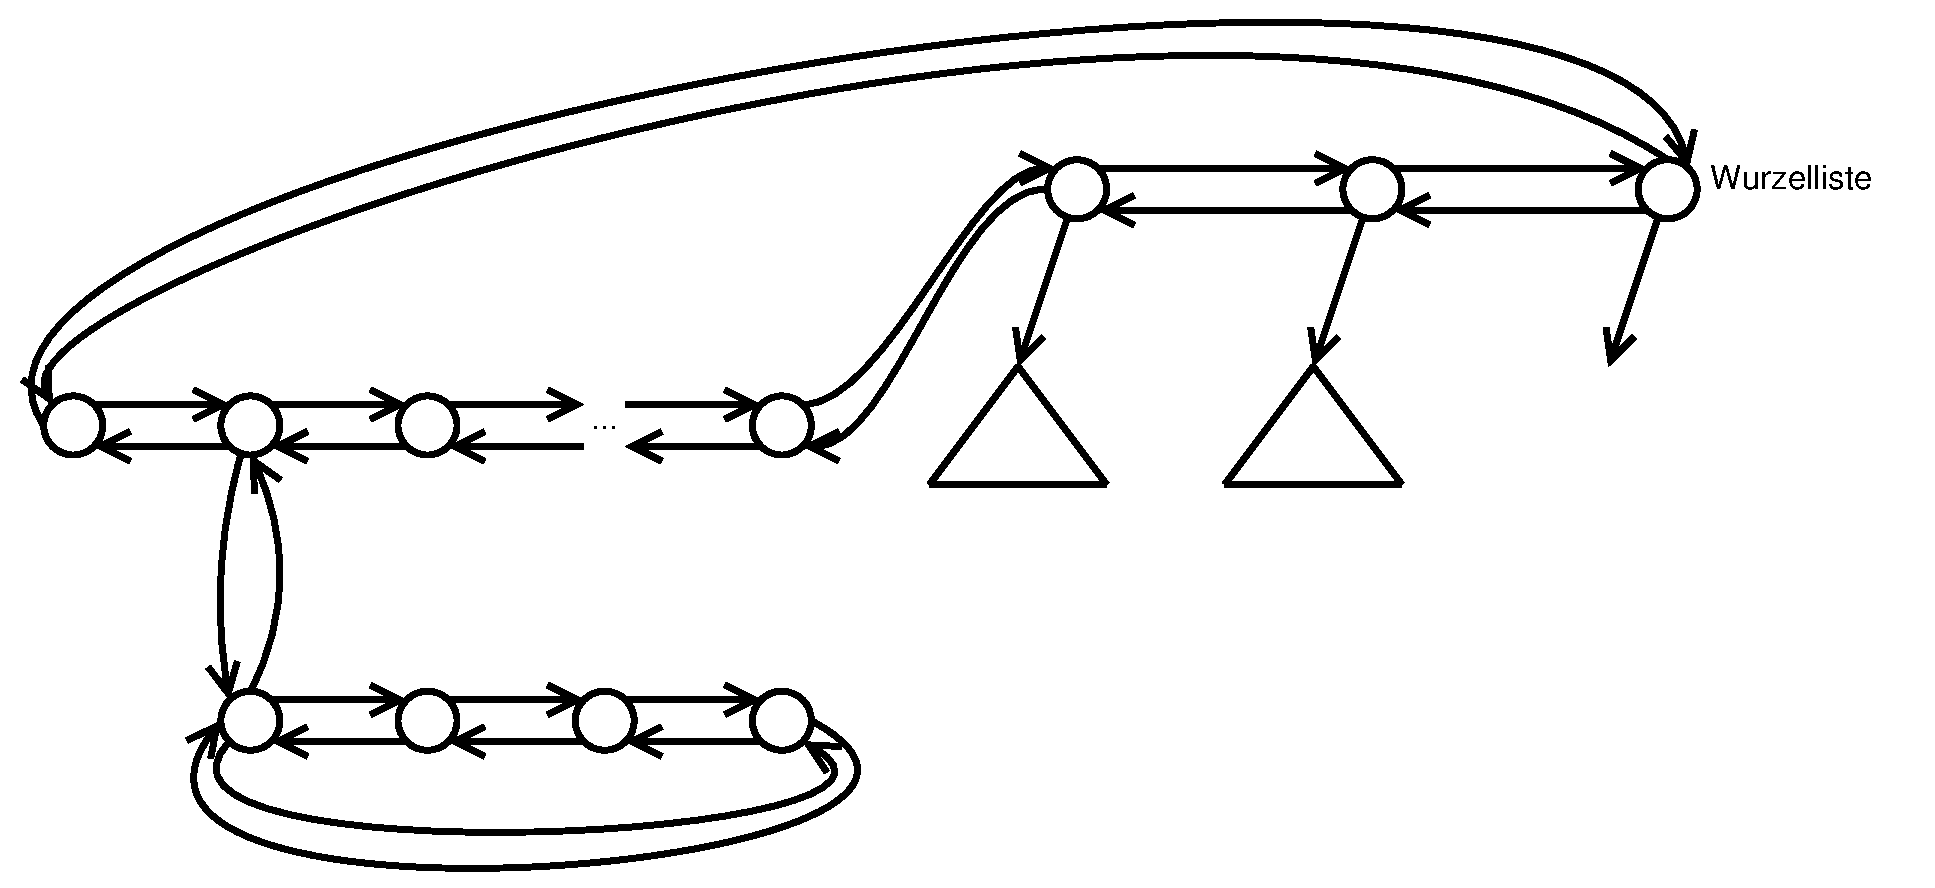
\includegraphics[width=0.65\linewidth]{21/Grafik/deleteMin}
	\caption{DeleteMin-Operation}
\end{figure}

\subsubsection{\texttt{decreaseKey}}
Wir können davon ausgehen, dass wir den betroffenen Knoten kennen. Falls der erniedrigte Schlüssel des Knotens kleiner als der Schlüssel des Vaterknotens wird, lösen wir den Knoten aus der Kindliste des Vaters und setzen ihn in die Wurzelliste. Wir markieren den Vater, dass er einen Kindknoten verloren hat. Sollte der Vater schon eine Markierung tragen, so wird auch der Vater Knoten abgelöst und in die Wurzelliste gesetzt. Dieser Prozess kann sich kaskadenartig bis zur jeweiligen Wurzel fortsetzen. Bei Aufnahme eines abgelösten Knotens in die Wurzelliste, muss auch das Minimum aktualisiert werden.

\begin{figure}[H]
\centering
\begin{subfigure}[h]{0.45\linewidth}
	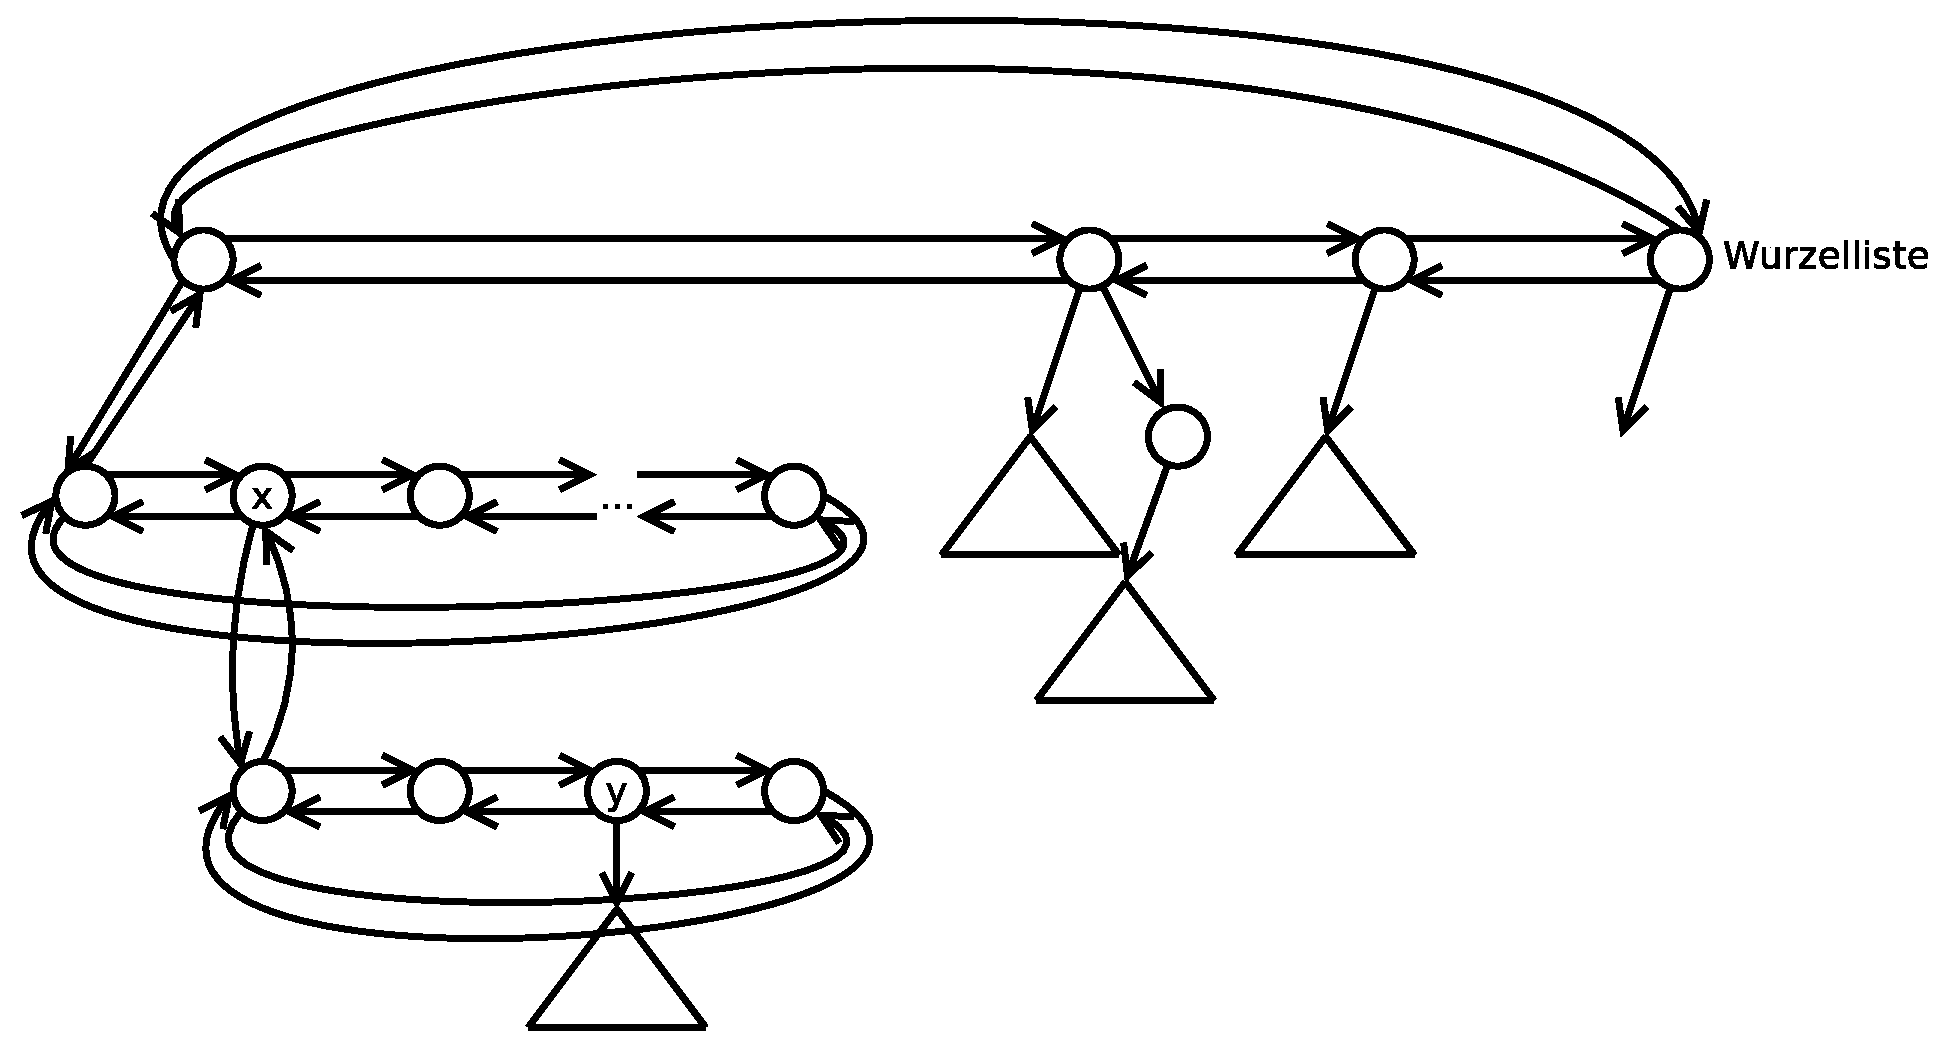
\includegraphics[width=\linewidth]{21/Grafik/decreaseKey1}
\end{subfigure}
\begin{subfigure}[h]{0.45\linewidth}
	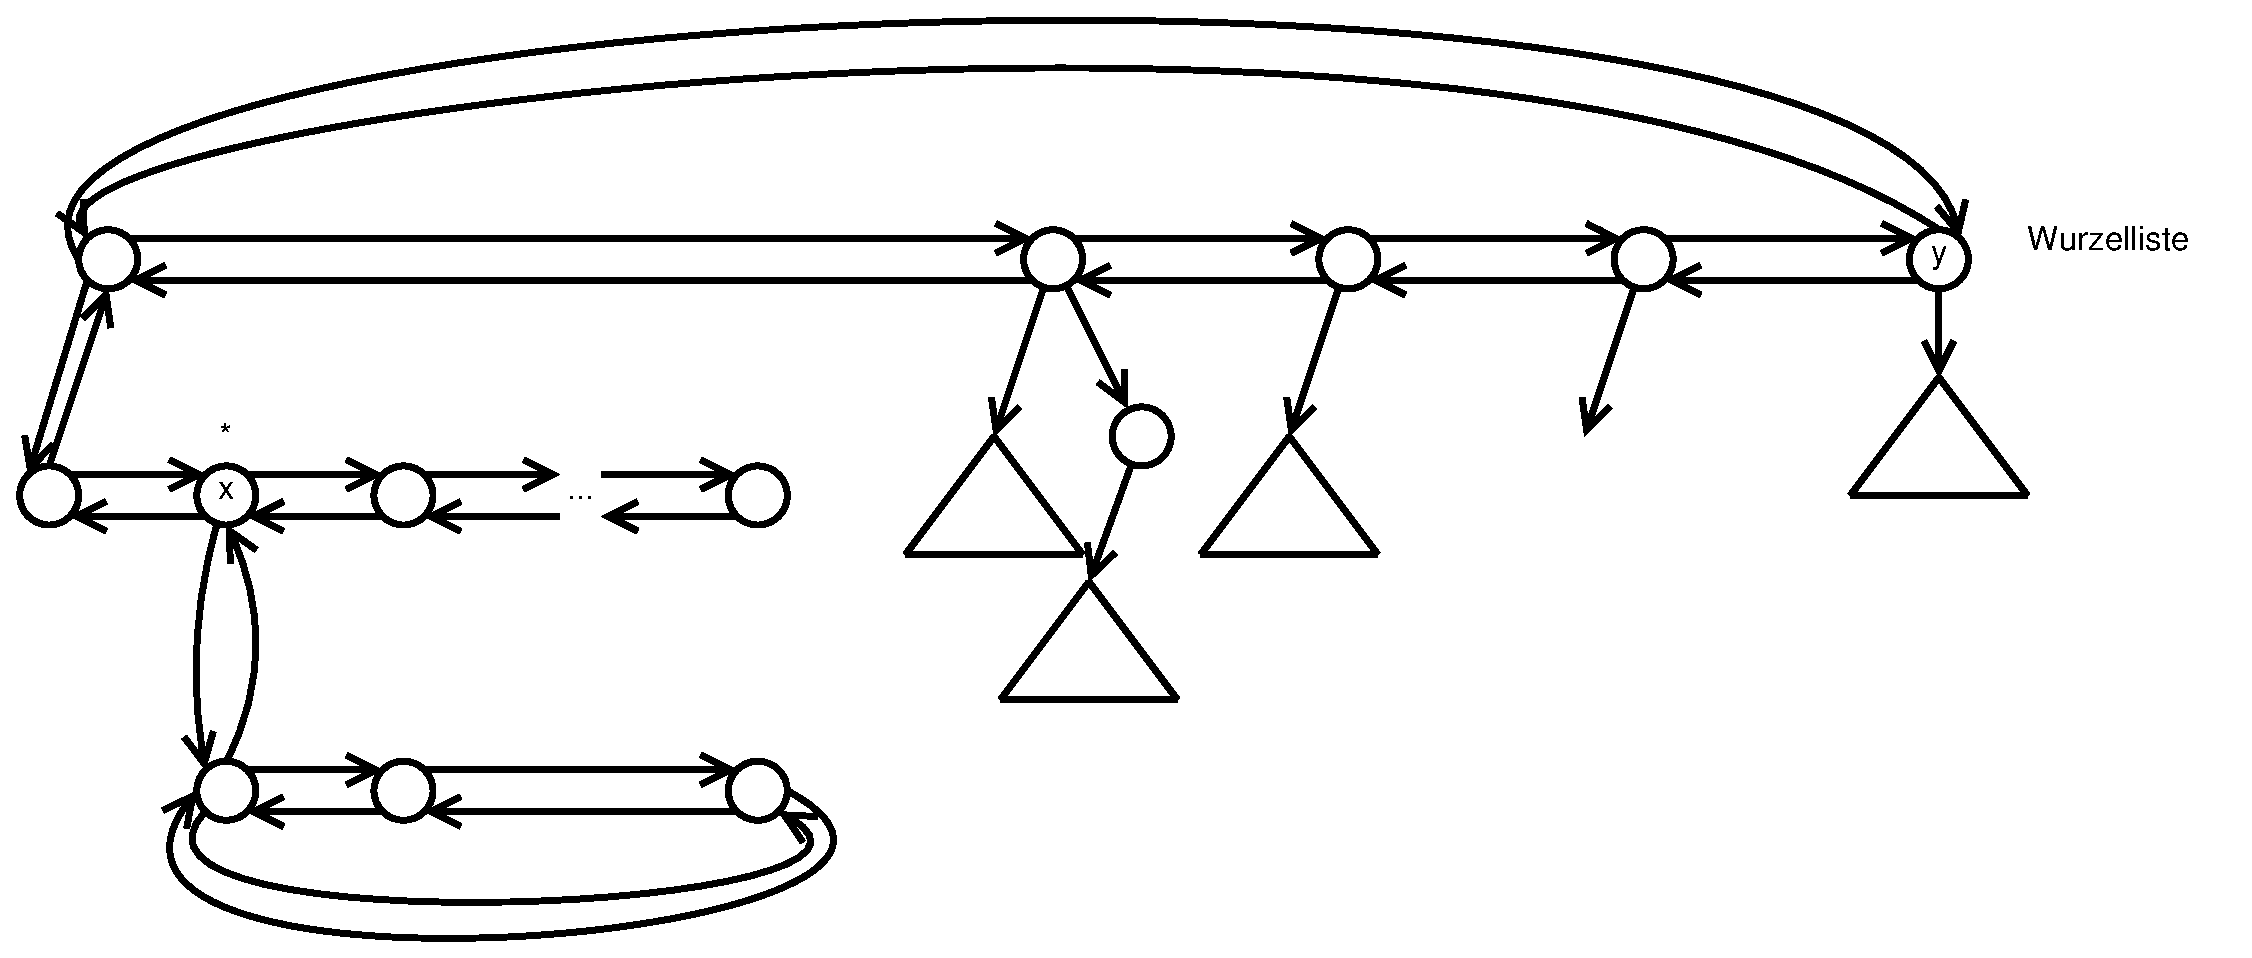
\includegraphics[width=\linewidth]{21/Grafik/decreaseKey2}
\end{subfigure}
\caption{decreaseKey-Operation}
\end{figure}

\subsubsection{Konsolidierung der Wurzelliste}
Nach dem "`Lazy Evaluation"'-Prinzip wird dieser Vorgang nur nach einem \texttt{deleteMin} angestoßen, um die Wurzelliste zu verkürzen. Wir nutzen ein einfaches Feld hinreichender Größe, um temporär Knoten, entsprechend ihren Grades, zu verwalten. Wir durchlaufen die Wurzelliste. Wenn wir einen Knoten vom Grad $k$ antreffen, schreiben wir ihn in das Feld an Position $k$ bzw. verschmelzen ihn mit dem Knoten von Grad $k$, den wir dort antreffen. Dadurch entsteht gegebenenfalls ein neuer Knoten vom Grad $k+1$ der an Position $k+1$ im Feld zu setzen ist. Es kann also zu weiteren Fusionsoperationen kommen. Analogie zu der Übertragungsfortpflanzung beim Binärzähler.

\begin{figure}[H]
	\centering
	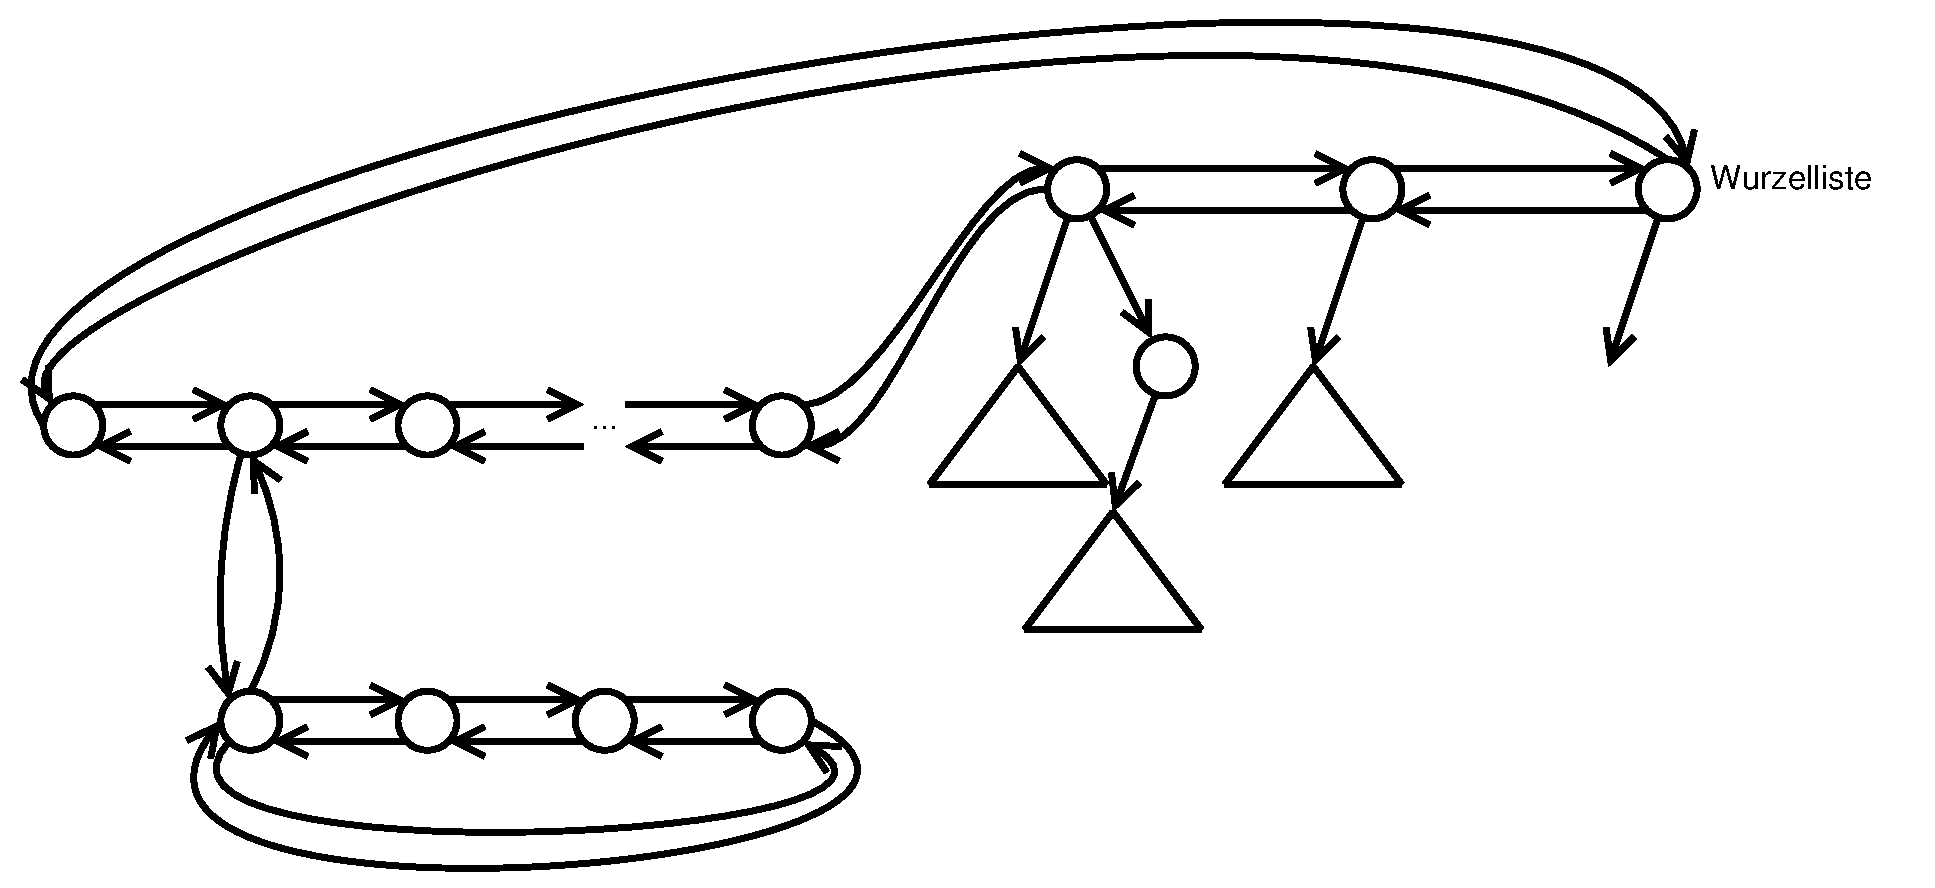
\includegraphics[width=0.65\linewidth]{21/Grafik/insert}
	\caption{Konsolidierungs-Operation}
\end{figure}

